\documentclass[crop,tikz]{standalone}

\usetikzlibrary{angles,calc}
\usepackage{pgfplots}
\pgfplotsset{compat=1.18}

\pgfplotsset{
  inverted/.style = {
    every axis legend/.append style={
      draw=white,
      fill=hardblack,
      text=white
    }
  },
}

\begin{document}
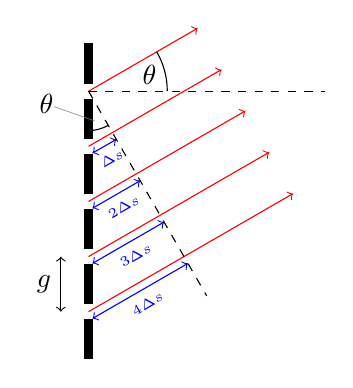
\begin{tikzpicture}
  \pgfmathsetmacro{\glength}{0.5};
  \pgfmathsetmacro{\gwidth}{0.1};
  \pgfmathsetmacro{\gdistance}{0.2};
  \pgfmathsetmacro{\g}{\glength + \gdistance};
  \pgfmathsetmacro{\angle}{30};
  \pgfmathsetmacro{\raylength}{3};
  % grating
  \foreach \m in {-1,...,4} {%
    \draw[fill] ({-\gwidth/2},{\m*\g + \gdistance/2}) rectangle ++ ({\gwidth},{\glength});
  }
  \begin{scope}[rotate={\angle}]
    % distances
    \draw[<->,blue] ({3*\g*sin(\angle)},{3*\g*cos(\angle)-0.1}) -- ++ ({\g*sin(\angle)},0) node[midway,below,rotate={\angle}] {\tiny $\Delta s$};
    \foreach \m in {2,...,4} {%
      \draw[<->,blue] ({(4-\m)*\g*sin(\angle)},{(4-\m)*\g*cos(\angle)-0.1}) -- ++ ({\m*\g*sin(\angle)},0) node[midway,below,rotate={\angle}] {\tiny $\m\Delta s$};
    }
    % rays
    \foreach \m in {0,...,4} {%
      \draw[red,->] ({\m*\g*sin(\angle)},{\m*\g*cos(\angle)}) -- ++ ({\raylength-\m*\g*sin(\angle)},0);
    }
  \end{scope}
  % angle 1
  \coordinate (O) at (0,{4*\g});
  \coordinate (R) at ($(O)+({\angle}:{\raylength+\g*sin(\angle)})$);
  \draw[dashed] (O) -- ++ ({\raylength},0) coordinate (A1);
  \pic[draw,pic text={$\theta$},angle radius=1cm,angle eccentricity=0.8] {angle = A1--O--R};
  % angle 2
  \coordinate (G) at (0,-1);
  \draw[dashed] (O) -- ++ ({-90+\angle}:{\raylength}) coordinate (A2);
  \pic[draw,pic text={},pic text options={pin={[pin distance=1.5em]170:{$\theta$}}},inner sep=0pt,angle radius=0.5cm,angle eccentricity=0.8] {angle = G--O--A2};
  % slit distance
  \draw[<->] (-1em,0) -- node[left] {$g$} ++ (0,{\g});
\end{tikzpicture}
\end{document}
